\documentclass[12pt, openany]{report}
\usepackage[utf8]{inputenc}
\usepackage[T1]{fontenc}
\usepackage[a4paper,left=2cm,right=2cm,top=2cm,bottom=2cm]{geometry}
\usepackage[frenchb]{babel}
\usepackage[pdftex]{graphicx}
\usepackage{amsmath,amsfonts,amssymb}
\usepackage{hyperref}
\usepackage{color}
\usepackage[table]{xcolor}
\usepackage{listings}
\usepackage{enumitem}
\usepackage{pifont}
\usepackage{ragged2e}
\usepackage{tabto}


\setlength{\parindent}{0cm}
\setlength{\parskip}{1ex plus 0.5ex minus 0.2ex}
\newcommand{\hsp}{\hspace{20pt}}
\newcommand{\HRule}{\rule{\linewidth}{0.5mm}}
%\renewcommand{\thesection}{\Roman{section}}
\renewcommand{\thesection}{\arabic{section}} 


%contenu du document
\begin{document}


\begin{titlepage}
  \begin{sffamily}
  \begin{center}
	
\includegraphics[scale=0.5]{ub.png}~\\[1cm]

    \textsc{\Large MASTER 2 Informatique RCI }\\[1.5cm]
    2021-2022

    % Titre
    \rule{1\linewidth}{2pt}
     \\[1cm]
    { \huge \bfseries Rapport de PFE :\\
    Déploiement d'un VPN sur des équipements mobiles ou IoT\\[1cm] }
    \rule{1\linewidth}{2pt}
    \\[1cm]
    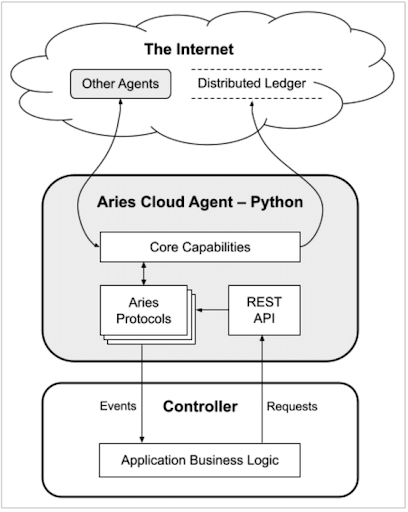
\includegraphics[scale=0.55]{couv.png}
    \\ %[1cm]

    % Membres du groupe
   \vfill
      \begin{center}
        %\hspace*{3.1cm}
        \Large	 Alexis Henquinet \hspace*{1cm} Mohamed Diallo \hspace*{1cm} Sara Real Santos
      \end{center}
 
    % Bas de la page
 
  \end{center}
  \end{sffamily}
\end{titlepage}

\newpage

\renewcommand{\contentsname}{Sommaire}
%\addcontentsline{toc}{section}{Remerciements}
\tableofcontents
\newpage

\section{Introduction}
\noindent 
\begin{flushleft}
L'apparition de l'Internet of Things permet de rendre nos vies quotidiennes plus accessibles. La quantité d'objets IoT augmente et continuera à le faire, avec des prédictions quantifiant le nombre de dispositifs IoT en 2025 à 25 millions, face à 4900 en 2015. Cependant, l'augmentation de l'utilisation d'objets IoT pose aussi des problèmes concernant la sécurité de ces dispositifs. En effet, beaucoup d'objets IoT sont vulnérables à des attaques, et de plus en plus, il y a des attaques visant spécialement les dispositifs IoT.\\ 
\vspace{5mm}
La plupart des dispositifs IoT ne sont pas protégés par manque d'espace dans la mémoire, ou alors nécessitent des mises à jour régulières pour pouvoir être protégés. Une façon de pouvoir sécuriser les échanges entre les composants d'un réseau IoT est d'utiliser un VPN afin d'encrypter les différents messages. Une autre mesure complémentaire concernant la sécurité des connexions est l'utilisation de certificats. Les certificats sont utilisés pour s'authentifier auprès de différentes entités. Les certificats permettent de sécuriser les connexions en vérifiant que le certificat soit signé par une autorité qui 'a notre confiance', et donc qui permet de démontrer que l'agent avec lequel nous communiquons est de 'confiance' et vice-versa. Cependant, ce système dépend des autorités de certification et peut présenter différents problèmes. D'une part la possible censure ou contrôle de la part de cette autorité, mais aussi le fait que si jamais cette autorité est attaquée, alors tout les certificats délivrés par celle-ci sont compromis. Pour pouvoir contrer ces difficultés, nous pouvons utiliser des systèmes décentralisés qui remplacent l'autorité de certification\\
\vspace{5mm}
Dans ce projet nous avons utilisé ces deux méthodes pour sécuriser les échanges IoT. Notre réseau IoT est composé d'une machine Android et une machine Debian. Nous avons aussi un serveur qui communique avec la Blockchain Indy qui authentifie les différentes parties, client et serveur. Dans les deux machines nous avons installé et configuré un VPN avec le software Wireguard. L'utilisation de certificats a été remplacée par l'utilisation de Verified Credentials et l'authentification auprès de noeuds Blockchain. \\

\end{flushleft}

\section{Étude de l'existant}
\noindent 
\begin{flushleft}
\subsection{Wireguard}
Wireguard est un VPN qui a été initialement déployé pour les systèmes Linux, mais qui maintenant peut être utilisé par des dispositifs Android, Windows, macOS et autres. Du côté utilisateur, Wireguard est simple à configurer. Il  suffit juste d'échanger des clés publiques et Wireguard configure le VPN. La clé publique est une clé de 32 bytes construite avec Curve25519. Wireguard utilise cette clé pour créer une interface réseau associé à la clé publique. Ces interfaces font partie de la 'cryptokey routing table', qui peut être configuré et à laquelle on peut ajouter des règles de routage supplémentaires. Quand des paquets sont envoyés vers une machine par un tunnel Wireguard (donc, par l'interface dans la cryptokey routing table), ils sont encryptés avec la clé publique de la machine qui reçoit le paquet.
Quand un 

\subsection{Verified Credentials}

\subsection{Aries }

\end{flushleft}

\section{Besoins}
\noindent 
\begin{flushleft}
TODO
\end{flushleft}
\subsection{Besoins fonctionnels}
\noindent 
\begin{flushleft}
TODO
\end{flushleft}
\subsection{Besoins utilisateurs non fonctionnels}
\noindent 
\begin{flushleft}
TODO
\end{flushleft}

\section{Scénarios fonctionnels}
\noindent 
\begin{flushleft}
TODO
\end{flushleft}

\section{Architecture et implémentation}
\noindent 
\begin{flushleft}
TODO
\end{flushleft}

\section{Analyse du fonctionnement \& Tests}
\noindent 
\begin{flushleft}
TODO
\end{flushleft}

\section{Conclusion}
\noindent 
\begin{flushleft}
TODO
\end{flushleft}
\subsection{Limitations}
\noindent 
\begin{flushleft}
TODO
\end{flushleft}
\subsection{Extensions}
\noindent 
\begin{flushleft}
TODO
\end{flushleft}

\section{Bibliographie}
\noindent 
\begin{flushleft}
TODO
\end{flushleft}

\section{Annexe}
\noindent 
\begin{flushleft}
TODO
\end{flushleft}
\end{document}

\begin{thebibliography}{}
\bibitem[1]{1}
https://www.wireguard.com/

\end{thebibliography}
